\chapter{Practical Part}
\subsection{Data Collection}
Actually, many datasets that contain images of hand gestures are publicly available to use. In this project, we recorded our data. We did so with the MediaPipe hand-tracking model. We achieved this by capturing camera footage of each gesture being held for a certain period of time and moving around for variety. During the capture process, we pressed a key to label each gesture. Our dataset consisted of over 5000 samples. The different hand conditions for dataset samples include images from both the right and left hand, palms facing forward or backward towards the camera, and various degrees of hand position captured by the camera.

 The model outputs x, y, and z coordinates of hand landmark points from images, with only x and y coordinates necessary and sufficient for training the final model. As a result, the z coordinates were eliminated, and the remaining x and y coordinates of hand landmarks for various hand signs are stored in a csv file for each hand landmark.  The coordinates in Figure \ref{fig:saved_csv} represent the data points used to generate the final dataset and train the final model. The first column represents the label of a gesture, the next two columns are coordinates of landmark 0 at the wrist, and so on. Csv contains many combinations of landmark coordinates for each gesture.


\begin{figure}
	\centering
	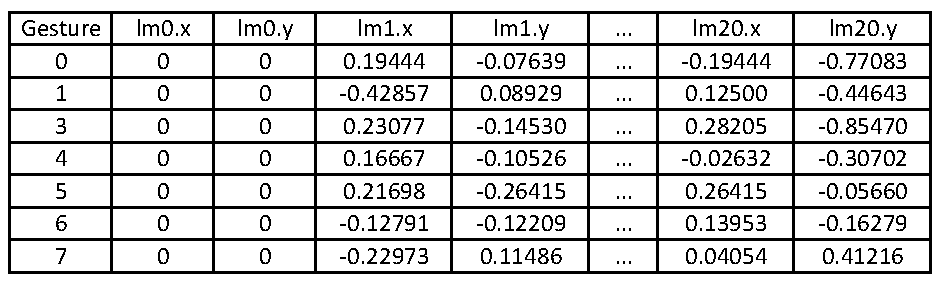
\includegraphics[width = \textwidth]{images/gesture_laandmarks-cropped.pdf}
	\caption{A selection of the saved csv file}
	\label{fig:saved_csv}
\end{figure}


\subsection{Model}

\subsubsection*{Training the Model}

2 modely na rozonavanie gest - aplm a landmark points\\


After creating the dataset, the next task is to train a feedforward neural network with the data.
We used an available model by MediaPipe. %SEM DAT NEJAKU REFERENCIU
The neural network (NN) has one input layer and one output layer, along with five hidden layers. These hidden layers include three dense layers and two dropout layers. The dense layers perform matrix-vector multiplication in the background, while the dropout layers reduce overfitting by randomly modifying the outgoing edges of hidden layer neurons and resetting them to 0 at each iteration during the training process.
The output layer of the NN has the same number of neurons as the possible hand gestures it can recognize. Each neuron represents a specific hand gesture and produces an output value indicating the probability of that gesture being present in the input.
Figure \ref{fig:layers} shows the model's configuration. The model was built using an Adam optimizer, which is efficient and suitable for training models with large data and parameters. The loss function used was Sparse Categorical Crossentropy, which measures the loss between actual and predicted labels. The accuracy metric was used to evaluate the model, indicating how often the prediction matches the actual label. The training model was initially set to have only 4 hidden layers, but the training accuracy didn't exceed 90\%. After updating to 5, without any other change, we got satisfactory results. The training accuracy obtained was 99.48\% and the calculated loss was 0.031.
\begin{figure}
	\centering
	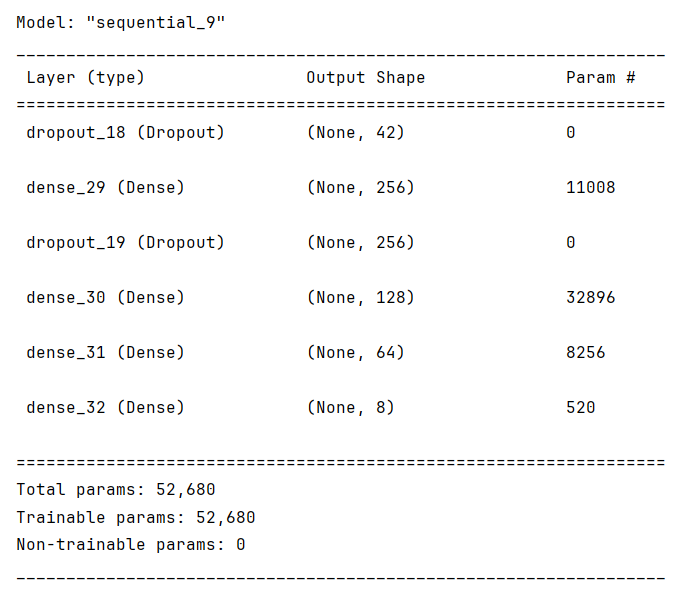
\includegraphics[width = 0.65\textwidth]{images/model_summ.png}
	\caption{Configuration of the used feedforward neural network}
	\label{fig:layers}
\end{figure}

\subsubsection*{Face Recognition Model}




\subsubsection*{Results and analysis of the model}

The  \text{classification\_report} and  \text{confusion\_matrix} libraries from scikit-learn were used for quantitative analysis of the test dataset. The \text{classification\_report} library produces an evaluation report of our model with accuracy, precision, recall, and F1 score matrices. Additionally, the 'support' matrix represents the model's real-time recognition performance.


\begin{figure}
	\centering
	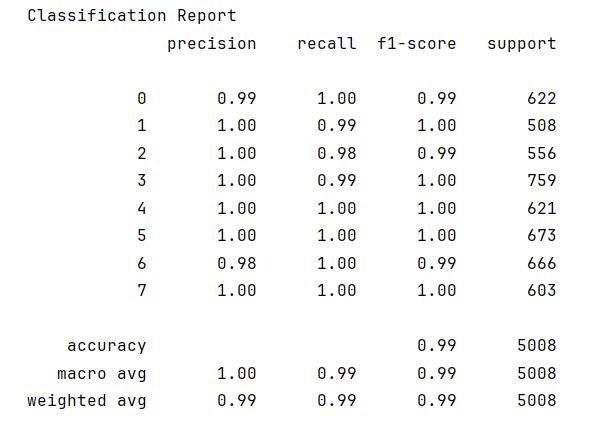
\includegraphics[width = 0.65\textwidth]{images/classific_report.png}
	\caption{Classification report of the model}
	\label{fig:report}
\end{figure}


Precision is the ratio of correctly predicted positive observations to the total predicted positive observations.

The accuracy matrix calculates the number of correctly predicted labels by the model from the entire dataset (Eq.\ref{eq:accuracy}). 
The precision matrix, on the other hand, measures the model's accuracy out of the predicted positives. It calculates the number of actual positives in the predicted positives and is an excellent measure to consider when the False Positive (FP) cost is high. Equation \ref{eq:precision} depicts the mathematical formula of the precision matrix.

The recall matrix measures the number of predictions our model correctly labels as positives. It is a measure considered when false negatives have high costs. The mathematical formulation of the recall matrix is Equation \ref{eq:recall}. 

The F1 score is calculated by combining both precision and recall, as shown in Equation \ref{eq:f1_score}. It is their harmonic mean.

Support is the number of samples in each class. 
The macro average of precision, recall and F1-score shows the average performance of the system across all classes, while the weighted average takes into account the class imbalance by weighting the metrics based on the number of samples in each class.
Additionally, the loss value of 0.0310 (not shown) indicates how well the model is minimizing its errors during training.

The classification report of the implemented model in detail is shown in Figure \ref{fig:report}. 


\begin{equation}
	\text{accuracy} = \frac{TP + TN}{TP + TN + FP +FN}
 \label{eq:accuracy}
\end{equation}

\begin{equation}
	\text{precision} = \frac{TP}{TP + FP}
  \label{eq:precision}
\end{equation}
\begin{equation}
	\text{recall} = \frac{TP}{TP + FN}
  \label{eq:recall}
\end{equation}

\begin{equation}
	\text{F1 score} = \frac{2 P  R}{P+ R} 
 \label{eq:f1_score}
\end{equation}

In the equations (\ref{eq:accuracy}), (\ref{eq:precision}), (\ref{eq:recall}), and (\ref{eq:f1_score}), TP, TN, FP, and FN represent True Positive, True Negative, False Positive,
and False Negative, respectively.

The confusion matrix is a performance measure used in machine learning, particularly in classification tasks. In Python, the scikit-learn library can be used to create a confusion matrix. To obtain the datasets for the experiment, we collected and pre-processed the data before using it to predict hand gestures. The confusion matrix was used to observe the accuracy achieved by the model. The confusion matrix of the used model is shown in Fig \ref{fig:confusion_matrix}. On the x-axis are predicted labels versus on the y-axis are actual labels.


Through the confusion matrix, we can determine which gestures are being recognized wrongly. For example, we can see that gesture 2 was 11 times misinterpreted as a gesture number 6. The recall of gesture 2 can then be calculated with Equation \ref{eq:recall2}:

\begin{equation}
	\text{recall(2)} = \frac{545}{545 + 11}
  \label{eq:recall2}
\end{equation}



\begin{figure}
	\centering
	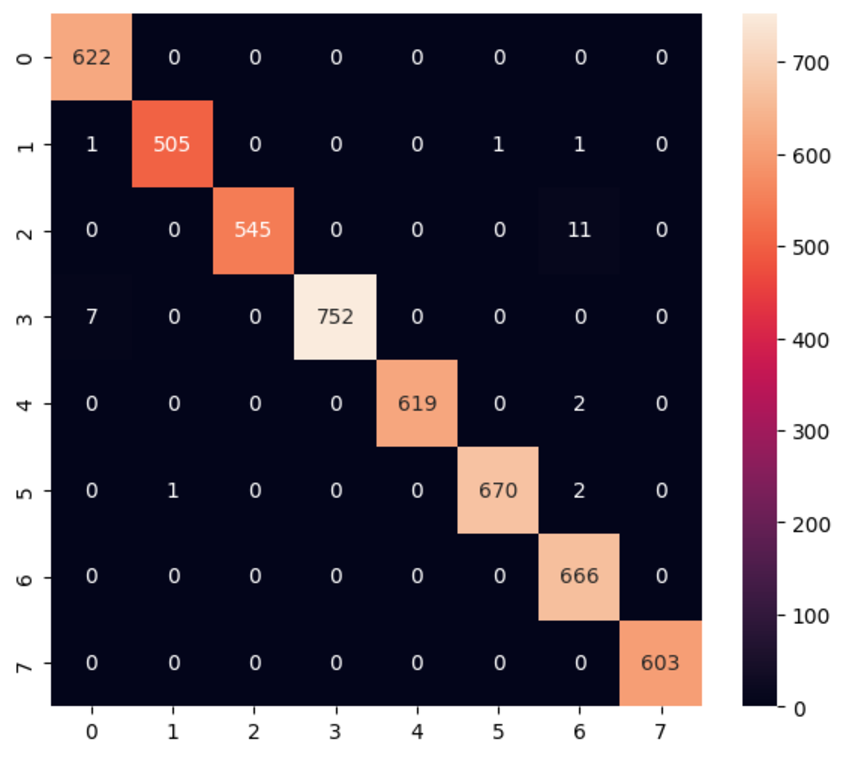
\includegraphics[width = 0.65\textwidth]{images/confusion_matrix.pdf}
	\caption{Confusion matrix of the model}
	\label{fig:confusion_matrix}
\end{figure}

The system's performance is satisfactory, with almost perfect precision, recall, and F1-score in most classes, as well as high accuracy and weighted average.

\subsection{Drone Implementation}

The Tello drone is a small quadcopter with a vision positioning system and an onboard camera. It is controlled by a laptop computer using Wi-Fi or a smartphone using 2.4 GHz. Using Python, it is easy to utilize the functions of the Tello library. This library has built-in functions for interacting with the drone, managing communication, handling state changes, and controlling the drone through a series of events.

In our program, Tello starts taking commands after a key press and recognizes a gesture every 5 seconds. This way it can comfortably execute a command before recognizing it again. After adjusting speeds and sleep times, the Tello drone executed the received commands practically immediately and consistently.

In table \ref{tab:gesture_commands} are displayed commands used in the project. We assigned them to the labels of our gestures. The gestures we use are shown in Fig \ref{fig:all_gestures} 


\begin{table}[ht]
\centering
\begin{tabular}{ll}
\toprule
Gesture Label & Command \\
\midrule
0 - Palm& Move along y-axis (forward velocity) \\
1 - Fist& Move along -y-axis (backward velocity) \\
2 - Rock& Flip forward (upward velocity) \\
3 - Ok & Take-off or land (depending on whether in flight or landed) \\
4 - Peace& Takes a picture (saves in png) \\
5 - Like& Rotate 360$^\circ$ \\
6 - Up& Move up (ascending velocity) \\
7 - Down & Move down (descending velocity)\\
\bottomrule
\end{tabular}
\caption{Gesture commands for drone control}
\label{tab:gesture_commands}
\end{table}

In addition, if we are not recognizing any gesture, the drone is ready to land on the palm. Because the drone can execute most of the commands only while flying, it takes off at the start of the program. It can also take off with gesture 4, so the program doesn't have to be reset.


